%%%%%%%%%%%%%%%%%%%%%%%%%%%%%%%%%%%%%%%%%%%%%%%%%%%%%%%%%%%%%%%%%%%%%%
%%                     Examples
%%%%%%%%%%%%%%%%%%%%%%%%%%%%%%%%%%%%%%%%%%%%%%%%%%%%%%%%%%%%%%%%%%%%%%

\chapter{Examples}


The following diagrams present examples of SBGN Activity Flow diagrams representing biological activities and their influences among each other in pathway networks.  They by no mean exhaust the possibilities of \SBGNAFLone.

\fig{TGF} presents an example of a signaling pathway involving the regulation of TGF$\beta$-induced metastasis.  The pathway was described in a report titled "A Mutant-p53/Smad Complex Opposes p63 to Empower TGF$\beta$-Induced Metastasis" in the April issue of Cell~\cite{Adorno:2009}.  The figure shows the usage of \glyph{biological activity nodes}, \glyph{phenotype}, \glyph{positive influence} arc, \glyph{negative influence} arc, \glyph{necessary stimulation} arc, and \glyph{logic operator}.

\begin{figure}
\begin{center}
\scalebox{0.5}{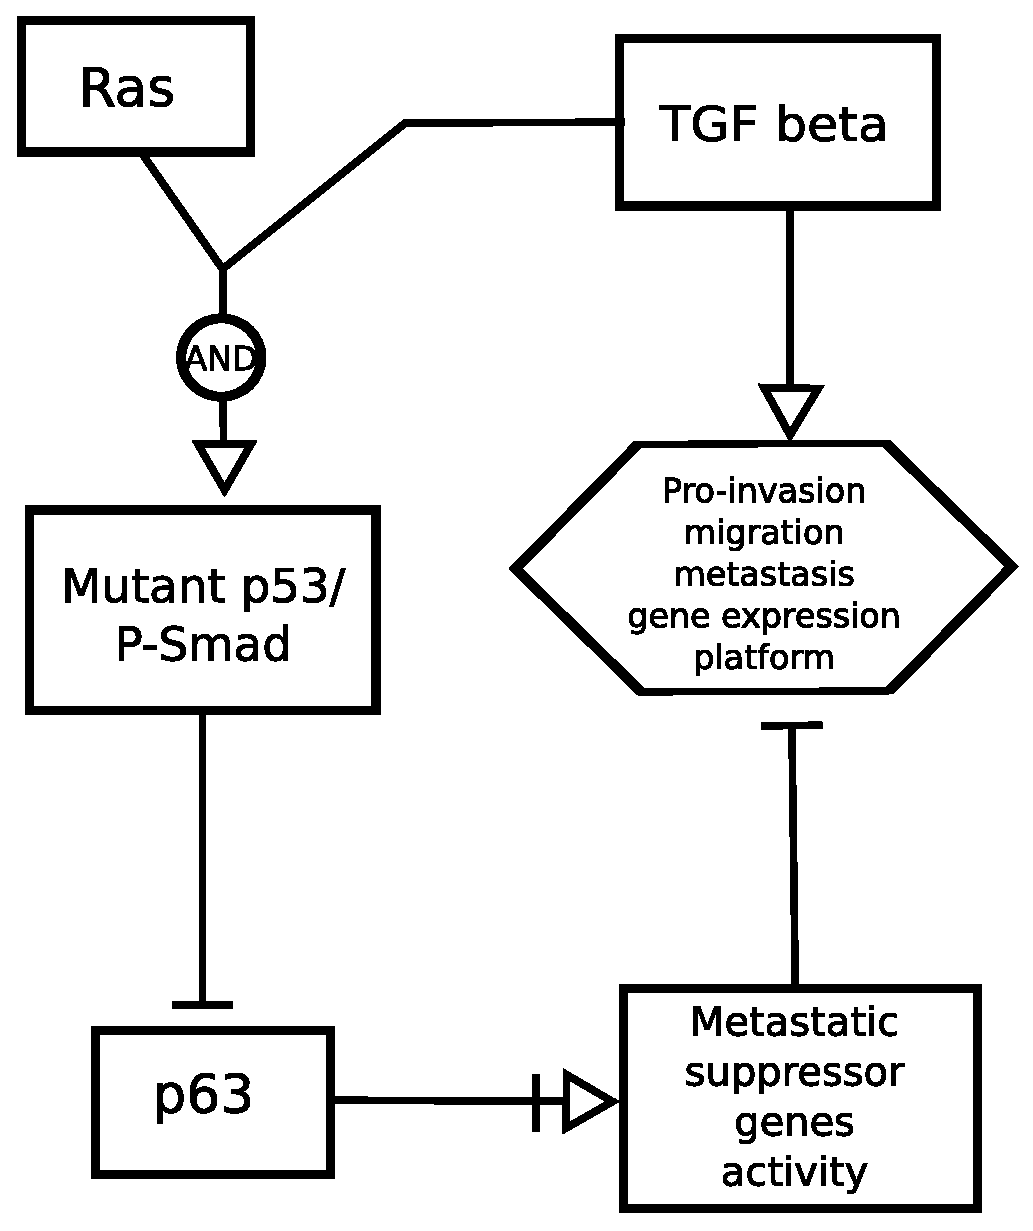
\includegraphics{examples/TGFbeta}}
\caption{Regulation of TGF$\beta$-induced metastasis.}\label{fig:TGF}
\end{center}
\end{figure}

\fig{EGF} presents a more complicated example of signaling pathway involving the intracellular signaling through the epidermal growth factor receptor (EGFR).  This example is a redraw of the Epidermal Growth Factor Receptor Pathway described in the Signal Transduction Knowledge Environment (\stkeurl).

\begin{figure}
\begin{center}
\scalebox{0.25}{\includegraphics{examples/EGFpathway}}
\caption{Epidermal Growth Factor Receptor Pathway.}\label{fig:EGF}
\end{center}
\end{figure}

\fig{TGFbeta} shows the transforming growth factor beta (TGF$\beta$) signaling pathway.  The map is a redraw of the TRG-beta Signaling Pathway described in the PANTHER Pathway System (\url{http://www.pantherdb.org/pathway/pathwayDiagram.jsp?catAccession=P00052}) and is based on reviews by Massague~\cite{Massague:1998} and Derynck~\cite{Derynck:2001}.

\begin{figure}
\begin{center}
\scalebox{0.40}{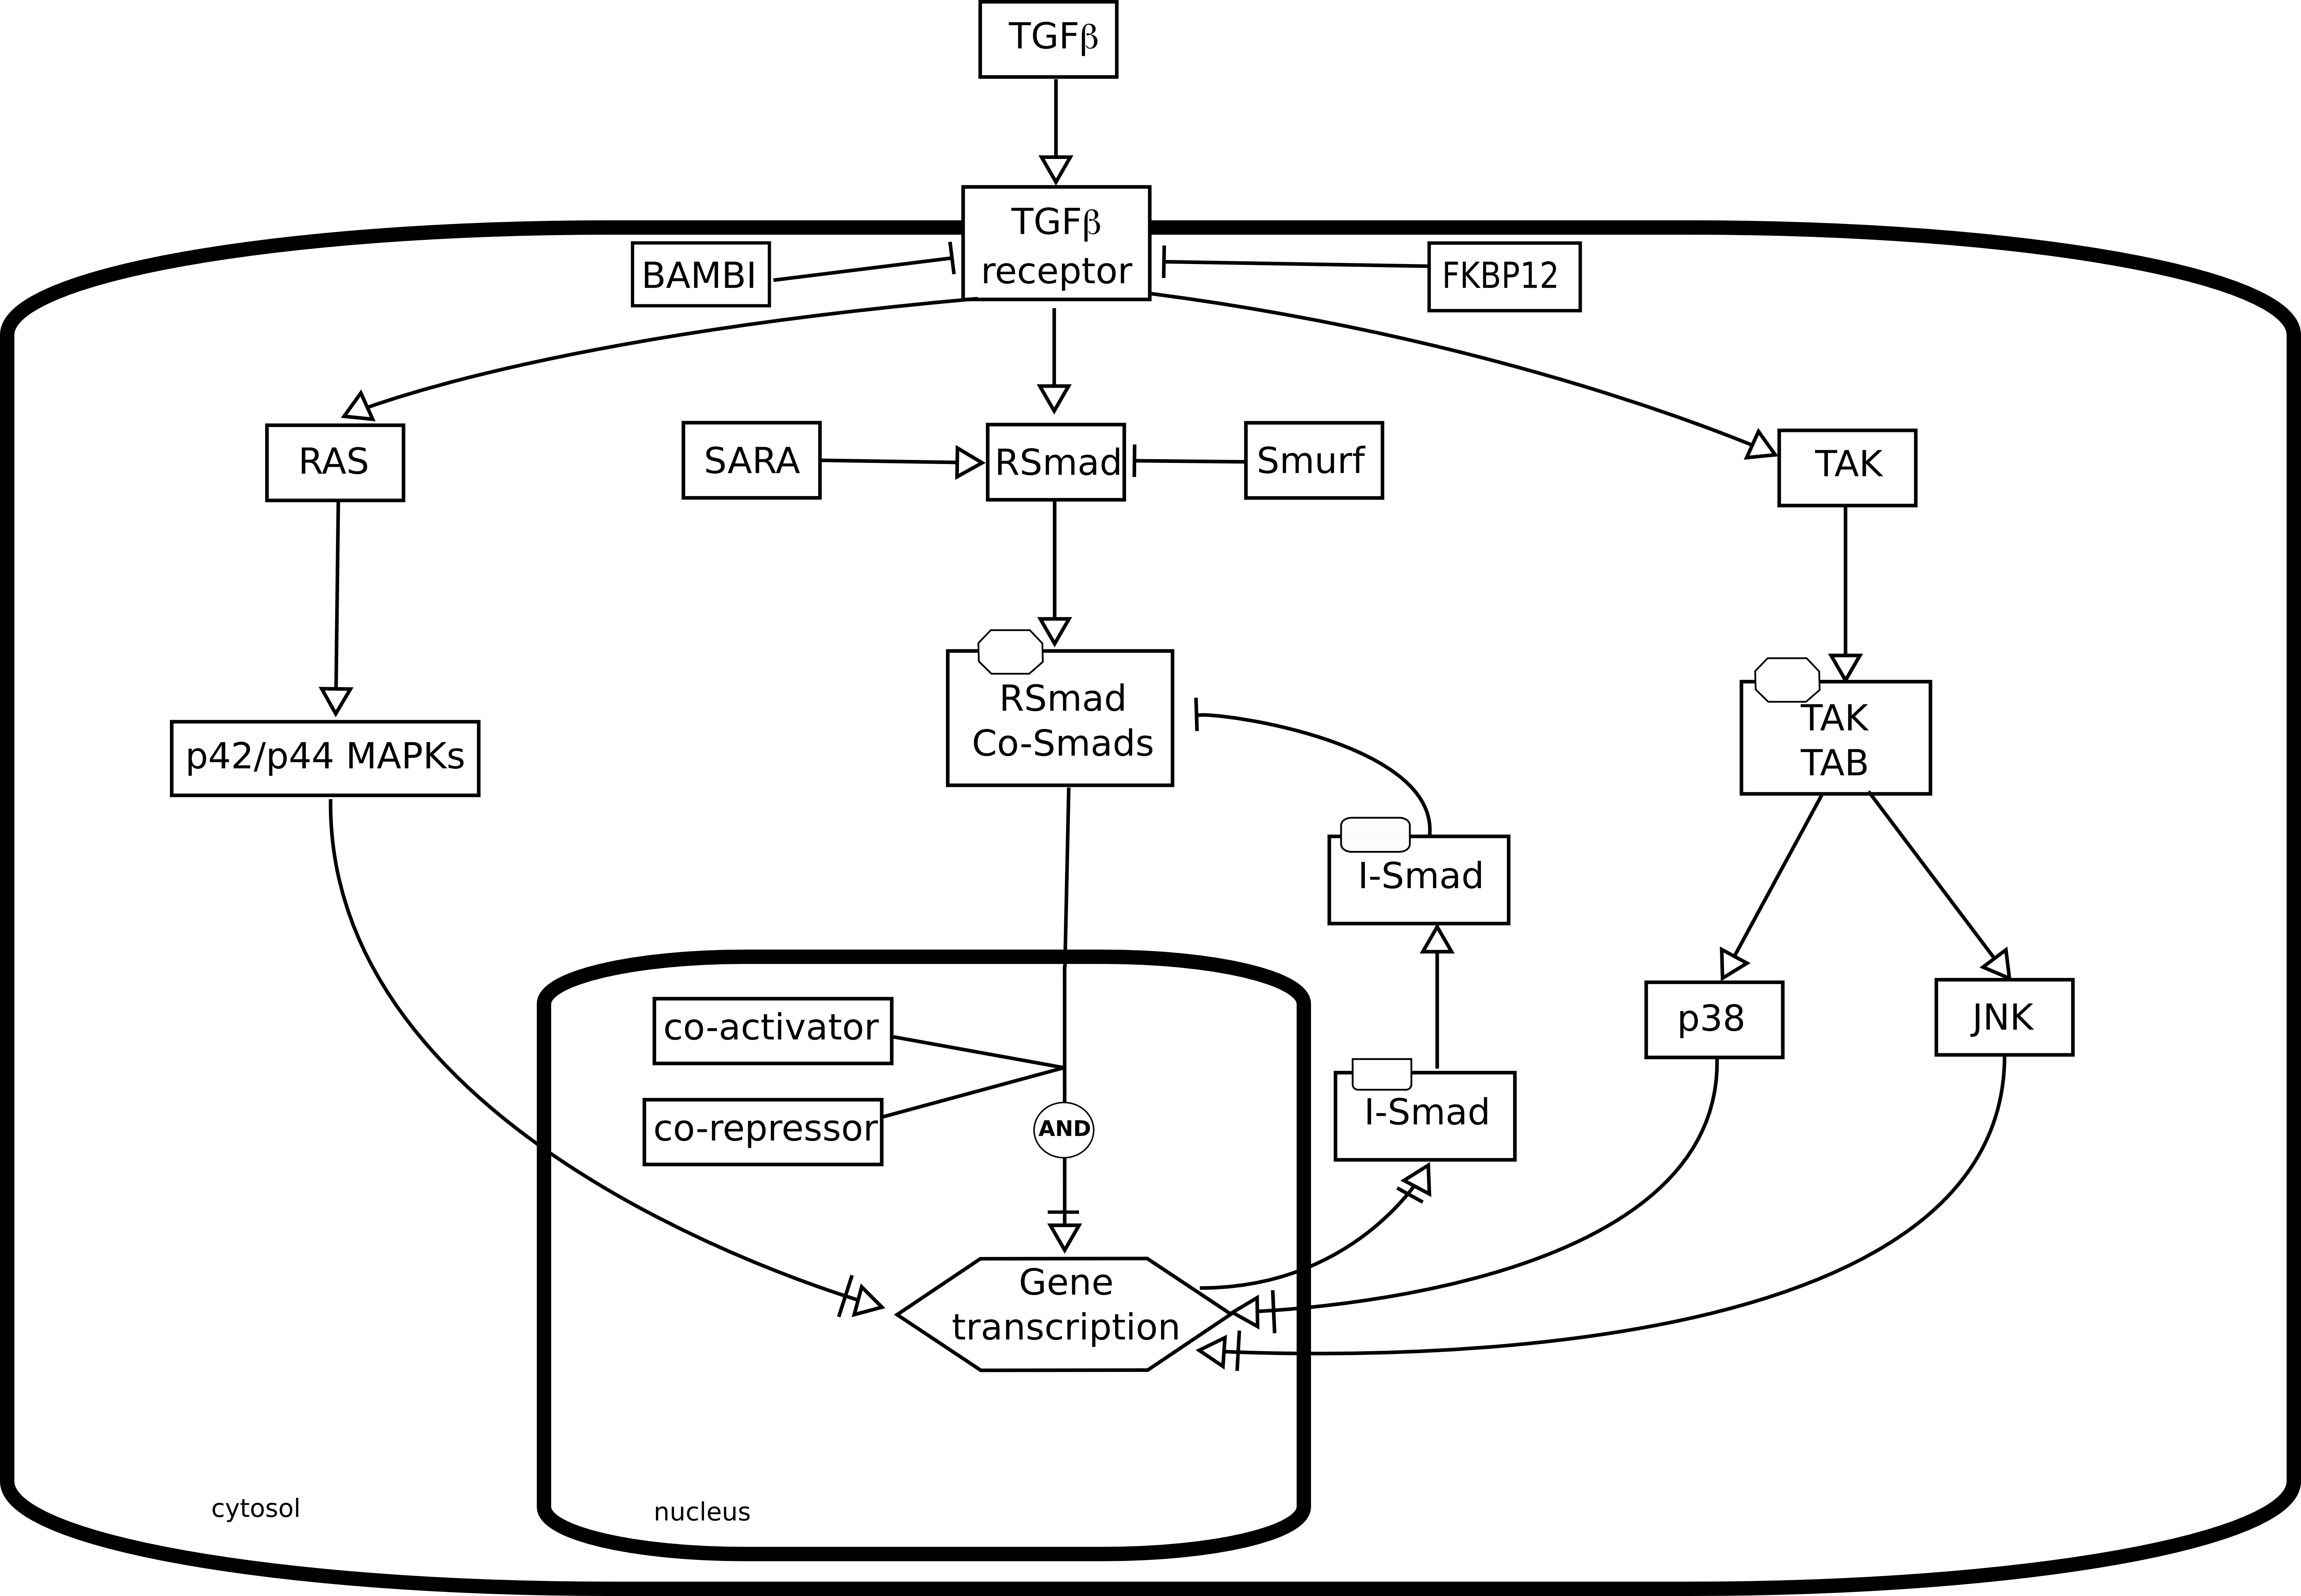
\includegraphics{examples/TGFbeta_pathway}}
\caption{Transforming Growth Factor beta signaling pathway.}\label{fig:TGFbeta}
\end{center}
\end{figure}

\fig{AP} presents the simplest view of action potential propagation mediated by the voltage-gated sodium channels.  There are two views how voltage-gated sodium channels are involved.  The diagram on the left side shows that the \glyph{increase in membrane potential} activates \glyph{voltage-gated sodium channel activity}, which in turn triggers membrane \glyph{depolarization}.  The diagram on the right side provides more detail in the mechanism.  It shows that the \glyph{increase in membrane potential} first activates the \glyph{gating activity} of the channel, which in turn activates the \glyph{conductance activity} leading to the membrane \glyph{depolarization}.  In this case, both \glyph{gating activity} and \glyph{conductance activity} come from the sodium channel gene, which is indicated as the \glyph{unit of information}.  In addition, this example also shows the advantage of using Activity Flow maps, because certain activities, such as gating and conductance, come from a number of amino acids in particular three dimensional structure that are not able to be illustrated in either Process Description or Entity Relationship maps.



\begin{figure}
\begin{center}
\scalebox{0.60}{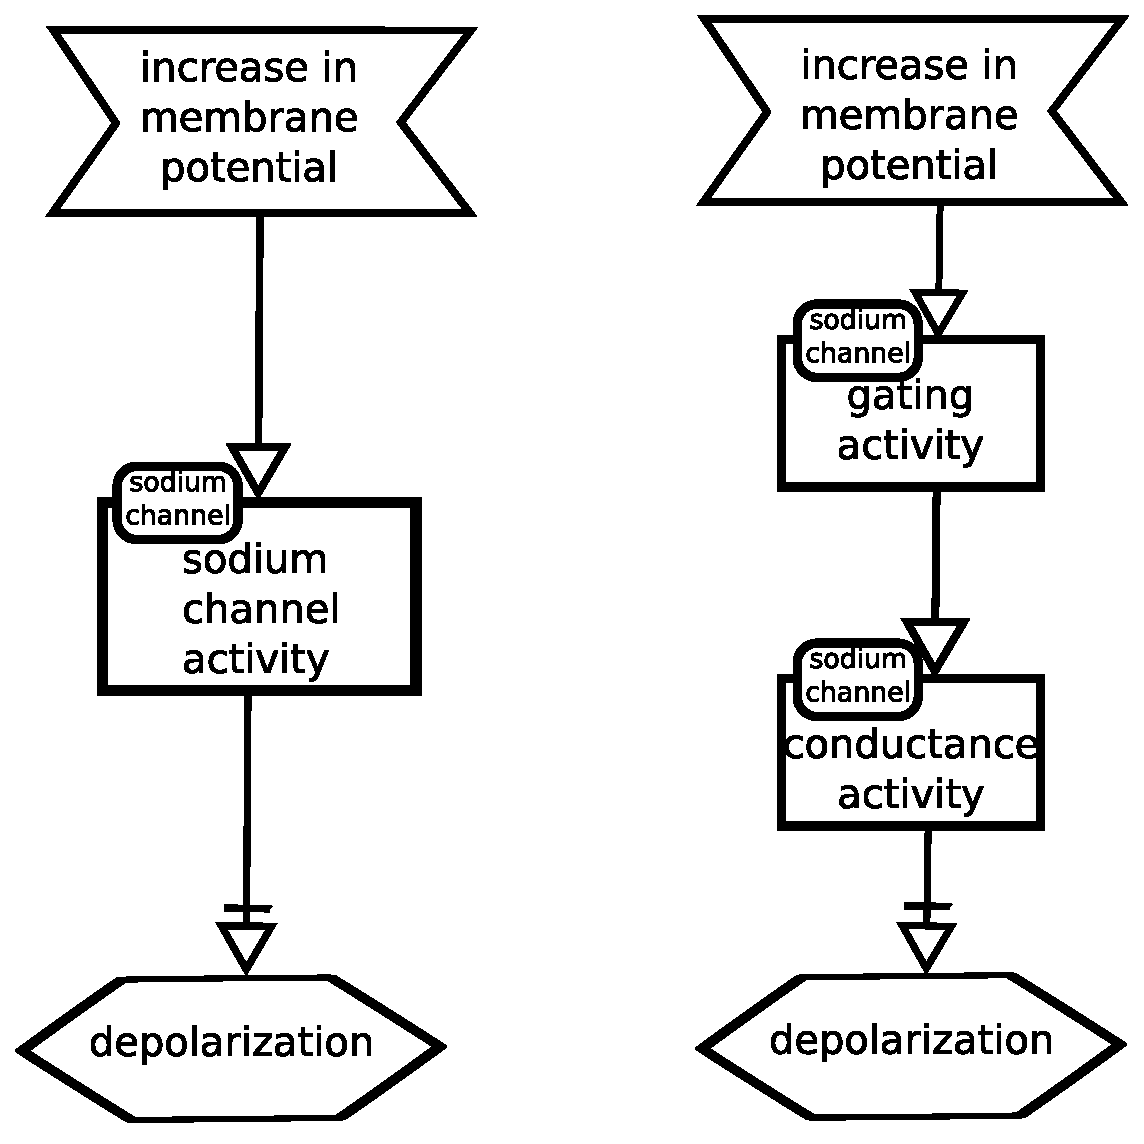
\includegraphics{examples/Action_potential}}
\caption{Two views of the role voltage-gated sodium channel plays in action potential generation illustrated by \SBGNAFLone.}\label{fig:AP}
\end{center}
\end{figure}















